% !TEX encoding = IsoLatin2  % notwendige Zeile für Mac-Benutzer (muss als Kommentar stehen); Windows-Benutzer können die Zeile löschen.

% LaTeX-Vorlage Version 3.1,  Juli 2011
% erstellt von Dr. Andreas Drauschke (andreas.drauschke@technikum-wien.at) und Dr. Susanne Teschl (susanne.teschl@technikum-wien.at)
% geringfügig adaptiert von Harald Stockinger (harald.stockinger@technikum-wien.at)

 
\documentclass[a4paper,bibtotoc,oneside]{scrbook} 
% Für kurze Arbeiten wäre auch die Dokumentklasse "scrartcl" ausreichend. In diesem Fall ist "section" die höchste Ebene ("chapter" gibt es dann nicht).
% \documentclass[a4paper,bibtotoc,oneside]{scrartcl}

%\usepackage{cclicenses}

% verlinkte Querverweise im pdf
\usepackage{hyperref}

% deutsche Anpassungen
\usepackage[utf8]{inputenc}
\usepackage[T1]{fontenc}
\usepackage[ngerman]{babel}


% mathematische Symbole
\usepackage{amsmath,amssymb,amsfonts,amstext}

% Kopfzeilen frei gestaltbar
\usepackage{fancyhdr}
\lfoot[\fancyplain{}{}]{\fancyplain{}{}}
\rfoot[\fancyplain{}{}]{\fancyplain{}{}}
\cfoot[\fancyplain{}{\footnotesize\thepage}]{\fancyplain{}{\footnotesize\thepage}}
\lhead[\fancyplain{}{\footnotesize\nouppercase\leftmark}]{\fancyplain{}{}}
\chead{}
\rhead[\fancyplain{}{}]{\fancyplain{}{\footnotesize\nouppercase\sc\leftmark}} 

% Farben im Dokument möglich
\usepackage{color}

% Schriftart Helvetica
\usepackage{helvet}
\renewcommand{\familydefault}{cmss} 

% Graphiken einbinden: hier für pdflatex
\usepackage[pdftex]{graphicx}

\usepackage{array}

% Höhe und Breite des Textkörpers etwas grösser definieren
\setlength{\textheight}{225mm}
\setlength{\textwidth}{1.05\textwidth}

% weniger Warnungen wegen überfüllter Boxen
\tolerance = 9999
\sloppy

% Anpassung einiger überschriften 
\renewcommand\figurename{Abbildung}
\renewcommand\tablename{Tabelle}

\begin{document}

% Kopf- und Fusszeilen initiieren
\pagestyle{fancy}
\pagenumbering{Alph}

% Deckblatt:
\thispagestyle{empty}
\begin{picture}(0,0)
\color{white}\sffamily
\put(-101,-749){
\includegraphics[width=1.002\paperwidth, height=\paperheight]{BM_2011.pdf}}
\put(220,-670){
\includegraphics[width=0.5\textwidth]{FHTW_Logo_4c.pdf}}
\put(-30, -20){\bfseries\huge BACHELORARBEIT}
% Titel des Studienganges einfügen:
\put(-30,-50){\Large im Studiengang Bachelor Informatik}
% Titel der Arbeit einfügen:
% Die Minipage wird gesetzt, damit auch mehrzeilige Titel möglich werden.
\put(-32,-150){
\begin{minipage}{14cm}
\bfseries\huge Software-Test von Web-Applikationen
\end{minipage}
}
% Name der Autorin/des Autors eingeben:
\put(-30,-250){\large Ausgeführt von: Bernhard Posselt}
% Personenkennzeichen der Autorin/des Autors eingeben:
\put(-30,-270){\large Personenkennzeichen: 1010257029}
% Name der Begutachterin/des Begutachters eingeben:
\put(-30,-310){\large Begutachter: MSc Benedikt Salzbrunn}
\put(-30,-350){\large Wien, \today} % das Datum des letzten Kompilierens wird automatisch eingesetzt
\color{black}
\end{picture}

\newpage


\section*{Eidesstattliche Erklärung}\thispagestyle{empty}
\glqq Ich erkläre hiermit an Eides statt, dass ich die vorliegende Arbeit selbständig angefertigt habe. 
Die aus fremden Quellen direkt oder indirekt übernommenen Gedanken sind als solche kenntlich gemacht. 
Die Arbeit wurde bisher weder in gleicher noch in ähnlicher Form einer anderen Prüfungsbehörde vorgelegt
und auch noch nicht veröffentlicht. Ich versichere, dass die abgegebene Version jener im Uploadtool entspricht.\grqq\\[5\baselineskip]
\rule{5cm}{0.2pt}\hfill\rule{5cm}{0.2pt}\\
\phantom{Datum }Ort, Datum\hfill Unterschrift\hspace{15mm}

\newpage


\section*{Kurzfassung}\thispagestyle{empty}
Die Durchführung und Erstellung von automatisierten Tests für Web-Applikationen unterscheidet sich von klassischen Applikationen. Aufgrund der komplexeren Infrastruktur und Modularisierung werden zusätzliche Testfälle und Strategien benötigt um Web-Applikationen ausreichend abzudecken und eine fortwährende Qualität zu gewährleisten. Diese Arbeit soll Möglichkeiten für den Test von Web-Applikationen aufzeigen.

\vfill
\paragraph*{Schlagwörter:} Webapplikationen, automatisierte Tests, Webtest


\newpage

\section*{Abstract}\thispagestyle{empty}
Creation and execution of automatic web application tests is different from tests of classic applications. A more complex infrastructure and modularisation require additional testcases and strategies to guarantee a good enough test coverage which in return ensures constant quality. This thesis highlights various possibilities to test web applications.

\vfill
\paragraph*{Keywords:} web applications, automatic tests, webtest
\newpage

%\section*{Danksagung}
%\thispagestyle{empty}
%Text Text Text Text Text Text Text Text Text Text Text Text Text Text Text Text
%\newpage

\tableofcontents\thispagestyle{empty}
\newpage

\pagenumbering{arabic}
\setcounter{page}{1}

% Falls die Kapitelüberschriften zu lang für die Kopfzeile oder das Inhaltsverzeichnis sind, so erzielt man
% dort Kurzformen der Kapitelbezeichnungen mittels:
% \chapter[Kurzform]{Lange überschrift}
\chapter{Einführung}

Durch die zunehmende Verbreitung von Smartphones und anderen mobilen Geräten erfährt der Markt für Software-Applikationen eine zunehmende Fragmentierung \cite{smartphone}[S. 1]. Viele dieser Plattformen erfordern das Erlernen von unterschiedlichen Programmiersprachen, Frameworks und Betriebssystemen \cite{android}\cite{ios}. Will ein/eine Software-EntwicklerIn eine Applikation plattformübergreifend anbieten, erfordert dies daher einen höheren Zeit- und Kostenaufwand.

Da viele dieser Mobilgeräte über einen Web-Browser verfügen, wird das Web als Applikations-Plattform immer attraktiver. Zudem erlauben Frameworks wie PhoneGap \cite{phonegap} dem/der EntwicklerIn eine plattformübergreifende Mobil-Applikation auf Basis von Web-Technologien zu erstellen, welche sich nahtlos in das System integrieren. 

\section{Problemstellung}
Aufgrund der Vielfalt an unterschiedlichen Web-Browsern erhöht sich jedoch auch der Testaufwand der Applikation. Die Browser implementieren die vom W3C vorgeschlagenen Standards ab und zu anders und in unterschiedlicher Geschwindigkeit. Nicht selten kommt es vor, dass gewisse Funktionen nur in einer eingeschränkten Auswahl von Web-Browsern voll funktionsfähig sind und zusätzliche Anpassungen erfordern. \cite{caniuse}

Ein weiteres Problem ist das verhaltene Upgradeverhalten der NutzerInnen. Im Falle des Internet Explorers 7 dauerte es mehr als 19 Monate bis rund die Hälfte der NutzerInnen auf die neue Version umgestiegen sind. \cite{insecure}[S. 3]


\section{Lösungsansatz}
Um eine konstante Qualität der Web-Applikation auf allen Plattformen zu gewährleisten, muss das bisherige Testssystem angepasst werden, um der höheren Komplexität von Web-Applikationen gerecht zu werden. 

Diese Bachelorarbeit soll die zusätzlichen Herausforderungen beim Testen von Web-Applikationen aufzeigen. Des Weiteren soll sie einen Überblick über mögliche Anwendungen und Anpassungen der drei häufigsten Testarten - den Unit Tests, Integration Tests, System Tests und Acceptance Tests - im Bereich der Web-Applikationen geben.


\section{Aufbau}
Kapitel 2 behandelt den Sinn und die Grenzen des Software-Tests und wie er sich in den Entwicklungsprozess einbinden lässt.

In Kapitel 3 wird auf die Unterschiede zwischen klassischen Applikationen und Web-Applikationen eingegangen. Dadurch sollen zusätzliche Probleme, die sich durch das Applikations-Modell ergeben, aufgezeigt werden.

Kapitel 4 beschreibt die Planung und den Ablauf des Testprozesses durch die Verwendung eines Testplanes.


Kapitel 5 beschäftigt sich näher mit dem praktischen Einsatz von Unit Tests, welche serverseitigen und clientseitigen Quellcode abdecken.

Kaptitel 6 nimmt sich des Themas des Integration Tests an und zeigt dessen Einsatzzweck bei Web-Applikationen.

Kaptitel 7 behandelt den Systemtest und dem Test der verschiedenen Plattformen.

Kapitel 8 beschäftigt sich mit dem Thema des Acceptance Tests und wie dieser bei Web-Applikationen umgesetzt werden kann.

\chapter{Warum testen}
Keine Applikation ist fehlerfrei\cite{empiric_invest}[S. 9]. Diese Fehler  führen nicht nur zu unzufriedenen Kunden, sondern auch zu hohen Kosten: \glqq Im Jahr 2000 wurde in den USA ein Schaden durch Softwarefehler in der Auto- und Flugzeugindustrie von 1,8 Milliarden US-Dollar errechnet. Dies entspricht ca. 16 \% des Softwareumsatzes.\grqq\cite{betrieb}[S. 15]

Die Fehler-Rate wird auf ungefähr 3 pro 1.000 Zeilen geschätzt, was bei einer aufwendigeren Applikation mit 100 Millionen Zeilen Quellcode eine durchschnittliche Anzahl von 300.000 Fehlern ergibt \cite{eval_regression}[S. 10]. 

Je früher diese Fehler entdeckt werden, desto kostengünstiger können diese beseitigt werden \cite{betrieb}[S. 17]. Daher ist es wichtig, möglichst früh mit dem Testen zu beginnen und den Software-Entwicklungsprozess dementsprechend anzupassen \cite{betrieb}[S. 16]. 

\section{Grenzen von Software-Tests}
Das Vorhandensein von Tests kann niemals eine komplett fehlerfreie Software garantieren, nur eine Abwesenheit von bestimmten Fehlern kann garantiert werden, nämlich jenen, die explizit mit Tests abgedeckt werden \cite{eval_regression}[S. 12]. Dies resultiert unter anderem daraus, dass die Anforderungen an die Software oft nicht komplett spezifiziert oder ungenau sind und die Komplexität der Applikation im Laufe der Entwicklung stark ansteigt. Zusätzlich können die Testfälle durch die vielen möglichen Eingaben lediglich einen kleinen Bereich der Funktionsweise abdecken \cite{software_qual}[S. 243].

Es ist jedoch nicht erstrebenswert, die ganze Applikation mit Tests abzudecken, da dies zu zu hohen Entwicklungskosten führen kann. Idealerweise werden daher nur jene kritischen Fälle mit Tests abgedeckt, deren Fehlerkosten die Kosten für die Erstellung der Tests übertreffen. \cite{eval_regression}[S. 12]

Die implementierten Testfälle müssen auch regelmäßig gewartet und aktualisiert werden, um ihre Effektivität zu gewährleisten, denn diese nimmt auf Dauer ab. Es ensteht eine sogenannte \glqq Testresistenz\grqq\\\cite{eval_regression}[S. 12], die daraus resultiert, dass die bestehenden Tests nur bekannte Fehlerfälle abdecken und neue mögliche Fehlerfälle nicht berücksichtigen. \cite{eval_regression}[S. 12-13]

\section{Vorteile von automatisierten Tests}
Da die vorhandenen Tests durch die Einbindung in den Entwicklungsprozess öfters durchgeführt werden müssen, kann sich durch das manuelle Testen der immer gleichen Tests schnell eine gewisse Eintönigkeit einstellen. Das wiederum kann unter anderem dazu führen, dass Tester bestimmte Tests nicht korrekt oder ineffizient ausführen. 

Dieses Problem kann durch eine Automatisierung des Testprozesses gelöst werden. Die Automatisierung erlaubt zudem bei zukünftigen Testdurchläufen eine Reduzierung auf ein Minimum des ursprünglichen Zeitaufwandes. Daher sollte versucht werden, möglichst viele dieser Tests zu automatisieren. \cite{test_auto}[S. 22-23]

Auch können automatisierte Tests rund um die Uhr ausgeführt werden, was eine effizientere Nutzung der Zeit garantiert.

\section{Testen im Projektmanagement}
Tests können jedoch nicht nur dazu verwendet werden, um Fehler in der Applikation zu finden, sondern auch um einen Überblick über den derzeitigen Stand der Implementation zu gewinnen: Sie geben dem/der EntwicklerIn und ProjektmanagerIn ein direktes Feedback über bereits korrekt implementierte Teile der Software-Spezifikation. Auch Milestones können durch Tests definiert werden. \cite{test_auto}[S. 2]

Zudem ist eine Abschätzung riskanter Bereiche möglich, die durch eine erhöhten Testbedarf bestimmter Bereiche offensichtlich wird. \cite{testing_apps_on_web}[S. 34]

\chapter{Unterschiede zu klassischer Software}
Im Gegensatz zu klassischen Desktop- oder Mobil-Applikationen bestehen Web-Applikationen wegen ihrer Client-Server-Architektur immer aus mehreren Modulen, die meist über ein Netzwerk miteinander verbunden sind, beispielsweise: 

\begin{itemize}
\item Datenbank-Server
\item Web-Server
\item Applikations-Server
\item Authentifizierungs-Server
\item Web-Browser
\end{itemize}

Durch diesen modularen Aufbau ist es besonders schwer einen Fehler zu lokalisieren. Ein Fehler kann z.B. durch einen Fehler im Quellcode des Applikations-Servers oder durch ein Netzwerkproblem entstanden sein. \cite{testing_apps_on_web}[Foreword]

Außerdem gibt es eine größere Vielfalt an Plattformen, auf welchen Web-Applikationen ausgeführt wird: Auf der Serverseite sind diese Plattformen noch vom/von der BetreiberIn festlegbar, sprich welches Betriebssystem und welche Datenbank eingesetzt wird, auf der Clientseite ist dies aber schon nicht mehr möglich. Die BesucherInnen der Webseite verwenden verschiedene Web-Browser auf verschiedenen Betriebssystemen, welche beide in unterschiedlichen Versionen vorliegen können. Auch können unterschiedliche Plugins und Fonts in unterschiedlichen Versionen installiert sein. \cite{testing_apps_on_web}[Foreword]

Zudem verlagert sich auch immer mehr Applikations-Logik von der Server- auf die Clientseite\cite{testing_apps_on_web}[S. 13]. Durch das Verwenden von \emph{Events}, welche unter anderem durch BenutzerInnen-Eingaben ausgelöst werden können, stellt clientseitiger Code eine größere Herausforderung für den/die TesterIn dar als Serverseitiger: Events können in unterschiedlicher Reihenfolge und Kombination auftreten, manche Aktionen lösen sogar mehrere Events aus. \cite{testing_apps_on_web}[S. 18]

Eine weitere Herausforderung stellt das Session Modell von Web-Applikationen dar: viele Web-Applikationen verwenden nur eine Session pro NutzerIn, erlauben aber mehrere gleichzeitige Logins. Werden mehrere Instanzen der Applikation gestartet - z.B. loggt sich der/die NutzerIn auf dem Mobiltelefon und dem Laptop auf der Webseite ein - kann dies zu Synchronisationsproblemen zwischen den einzelnen Instanzen führen: Wird in einer Instanz ein Eintrag gelöscht, kann dieser durch eine fehlerhafte Synchronisation in einer andere Instanz immer noch existieren und in weiterer Folge zu Fehlern führen. \cite{testing_apps_on_web}[S. 20]

Diese Vielfalt an verschiedenen möglichen Konfigurationen und Herausforderungen erfordert eine neue Herangehensweise an das Thema Software-Test: Die bestehenden Techniken sind \glqq zwar auch notwendig, aber nicht ausreichend, um die Qualität der Applikation sicherzustellen\grqq\ \cite{eval_automat_webapp_test}[S. 18]


\chapter{Testplan}
Mit dem Erstellen des Projektplanes sollte gleichzeitig auch ein Testplan erstellt werden \cite{eval_automat_webapp_test}[S. 24]. Dieser erlaubt, den Testprozess näher zu spezifizieren und somit den erforderlichen Aufwand besser abschätzen zu können \cite{test_large_systems}[S. 18] und den Testprozess eventuell an ein externes Team auszulagern. Zusätzlich kann der Plan auch dazu verwendet werden, die Abnahmekriterien exakt zu definieren, um das Projektrisiko zu verringern. \cite{eval_automat_webapp_test}[S. 26]

Im Testplan werden unter anderem folgende Punkte behandelt \cite{test_auto}[S. 3]:

\begin{itemize}
	\item Was wird getestet? Welche Bereiche besitzen eine höhere Priorität als andere?
	\item Wo wird getestet? Mit welchen Konfigurationen, Soft- und Hardware Plattformen respektive Versionen werden getestet?
	\item Wie wird getestet? mit welchen Tools wird getestet?
	\item Wer testet?
	\item Wie lange wird getestet? Bis wann muss ein Test erfolgreich absolviert werden?
	\item Was wird nicht getestet?
\end{itemize}

Der Testplan wächst mit dem Projekt und muss demensprechend regelmäßig auf Korrektheit und Angemessenheit überprüft werden. \cite{eval_regression}[S. 25] 

Um den Ablauf der Tests zu beschleunigen, sollten unnötige Testdurchläufe vermieden werden. Dies wird mit der Erstellung eines Smoke-Tests erreicht der essentielle Testszenarien durchtestet. Schlagen diese fehl, sind weitere Testdurchläufe nicht notwendig und der Testdurchlauf kann abgebrochen werden. \cite{eval_regression}[S. 25-26]


\section{Vorteile eines Testplans}

Da die Entwicklung der Applikation meistens mit einem hohen Zeitdruck verbunden ist\cite{software_qual}[S. 244], ist es wichtig, bestimmte Testfälle höher zu priorisieren als andere \cite{testing_apps_on_web}[S. 34]. Dazu werden alle essentiellen Testfälle herausgearbeitet und dokumentiert. Aufgrund der Dokumentation der Testfälle, ergeben sich zusätzlich folgende Vorteile:

\begin{itemize}
	\item Fehlende Testfälle können schnell erkannt werden \cite{test_large_systems}[S. 18]
	\item Redundante Testfälle werden identifziert, Testfälle können zusammegelegt werden um Zeit zu sparen \cite{testing_apps_on_web}[S. 34]
	\item Verschiedene Testbereiche können an mehrere Personen mit unterschiedlichen Fachkenntnissen verteilt werden um Personalengpässe zu vermeiden \cite{test_large_systems}[S. 19]
	\item Ineffiziente Test-Tools und Test-Strategien können erkannt und verbessert werden \cite{eval_regression}[S. 25]
	\item Geschäftskritische Bereiche und solche mit einer erhöhten  Fehleranfälligkeit werden sichtbarer \cite{testing_apps_on_web}[S. 34]. Dies ist vor allem wichtig, da Fehler ungleich verteilt sind und in bestimmten Bereichen häufiger vorkommen als in anderen \cite{eval_regression}[S. 12]
	\item Sinnlose Testfälle und Testbereiche können aussortiert werden 
	\item Abhängigkeiten der Testfälle untereinander und der Implementation werden transparent und erlauben schnell auf Änderungen zu reagieren\cite{test_auto}[S. 4]
\end{itemize}


\chapter{Unit Test}
% Tested module und komponenten kleinste teile und routinen der software
% erlaubt eine reduzierung der komplexität und aufspalten in kleinere probleme
% erlaubt frühes testen da keine kompletten module da sein müssen
% zeigt schwer zu verwendende interfaces auf
% Schnell und genau ausführbar
% Isoliert und unabhängigkeit von einander ausführbar erlaubt paralellisierung
% wird vom entwickler der daran arbeitet selbst durchgeführt
% überprüft die spezifikation einer methoden/funktion
% kann keine kommunikation testen, abhängigkeiten werden mit mocks ersetzt
%\cite{test_large_systems}[S. 52]


% whitebox test sprich quellcode und implementation ist bekannt
%\cite{betrieb}[S. 26]

% todo: beispiel phpunit test, jasmine test

\chapter{Integration Test}
% Tested Subsysteme (beinhaltet merhere module), Diese Subsysteme werden dann auch zusammengesetzt und zusammengetestet
% da unittest schon genauen funktionen getestet hat richtet sich der integration test eher an die kommunikation zw. den elementen und deren interfaces
% kann in inkrementelle tests und nicht inkrementelle tests (vorgehensorientierte, zieldefinierte) aufgespaltet werden (sprich ob jedes modul einzeln getestet wird oder die module auf die vorigen getestet module a)
%\cite{test_large_systems}[S. 53-54]

% kann nicht durch unittests ersetzt werden
%\cite{betrieb}[S. 28]

% Gibt keine allgemeingültige strategie, hängt von projekt ab
%\cite{betrieb}[S. 29]

% todo: phpunit integration test, jasmine integration test

\chapter{System Test}

% testet das gesamtsystem 
% funktionale und nicht funktionale tests aber eher nicht funktionale \cite{test_large_systems}[S. 60]
% auf installationsumgebung getestet
% oft schwierig weil es auf produktivsystem des kunden läuft
% testet abläufe auf unterschiedlichen betriebssystemen + configs
% installation
% security
% 
%\cite{betrieb}[S. 30-31]

% manueller test möglich, die dokumentation kann auch damit durchgetestet werden
%
%\cite{test_large_systems}[S. 60]


% todo: gherkin + chef beispiele

\chapter{Acceptance Test}

% test von kunden auf vertragliche richtlinien, oft stark kunde miteinbezogen
% benutzbarkeit

%\cite{eval_regression}[S. 28]
%
%\cite{test_auto}[S. 11]
%
%Development acceptance tests:
% data driven \cite{test_auto}[S. 24]
% * Release acceptance tests (smoke tests): mainstream data + mainstream funktionen \cite{testing_apps_on_web}[S. 36]
% * Functional acceptance simple test: each dev release to test accessibility of key features on minimum configuration, no full functionality test (file saving example) \cite{testing_apps_on_web}[S. 37-38]

%Deployment acceptance tests:
%Full installation + configurations
% * Task-Oriented Functional Test: Features test (gherkin) against requirements, specs + design docs \cite{testing_apps_on_web}[S. 42]
% * Forced Error Test: testing for failures 
% * boundary test: test extreme inputs
% * system level test: test whole application \cite{testing_apps_on_web}[S. 43]
% * real world user level test: echte leute testen um fehler zu finden die man sonst übersieht
% * exploratory test: überlegen wo es probleme geben könnte und dort testen
% * stress test: limited resource conditions (memory, diskspace, network bandwidth)
% * Performance tests: testen wieviel das system verträgt
% * Regression tests: für bugs die schonmal aufgetreten sind \cite{testing_apps_on_web}[S. 44]
% * Compability + config tests: testen auf unterschiedlichen platformen
% * documentation test: testen von zb shortcuts \cite{testing_apps_on_web}[S. 45]
% * install uninstall test
% * UX tests
% * External beta tests \cite{testing_apps_on_web}[S. 46]
% * Secuirty tests
% * Unit tests
%\cite{test_large_systems}[S. 10]

%test ist mehr als simples aufnehmen und abspielen von inputs: ist redundant und eintönig, muss automatisiert werden muss geplant werden und auch generisch sein ansonsten braucht wartung der test skripte mehr aufwand und reibereien mit kollegen wenn sie etwas ändern
%automatisiertes monkey testing findet nur absturz bugs aber keine funktionalen bugs 


\chapter{Zusammenfassung}
% \cite{process_oop}[S. 30]


%\\[2\baselineskip]
%Hier wird auf Abbildung~\ref{Abb1} verwiesen. 
%\begin{figure}[htbp]
%\centering
%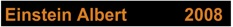
\includegraphics[width=75mm]{Buchruecken}
%\caption[Beschriftung eines Buchrückens.]{Beispiel für die Beschriftung eines
%Buchrückens.}\label{Abb1}
%\end{figure}
%%Tabelle~\ref{Tab1} ist ein Beispiel dafür, wie eine Tabelle aussehen könnte.
%\begin{table}[htbp]
%\centering
%\begin{tabular}{ | c | c | c | }\hline
%{\bf Datum} & {\bf Thema} & {\bf Raum}\\ \hline
%\hline
%20. 08. 2008 & Graphentheorie & HS 3.13\\ \hline
%01. 10. 2008 & Biomathematik & HS 1.05\\ \hline
%\end{tabular}
%\caption[Semesterplan "`Angewandte Mathematik"'.]{Beispiel für einen
%Semesterplan "`Angewandte Mathematik"'.}\label{Tab1}
%\end{table}

%\noindent
%Nun ein Beispiel für eine abgesetzte Formel:
%\begin{equation}
%x =  - \frac{p}{2} \pm \sqrt{\left(\frac{p}{2}\right)^2 - q}.
%\end{equation}
%Und eine mehrzeilige Formel:
%\begin{eqnarray}
%f(t)&=& t^2 \label{For1},\\
%g(t) &=& t-1.
%\end{eqnarray}
%Hier wird auf die Formel (\ref{For1}) verwiesen. \\

%\noindent
%So kann zum Beispiel ein \glqq Source-Code\grqq\  angegeben werden: 
%\begin{verbatim}
%for (i=1; i < 10; i++) {...} 
%\end{verbatim}

%\noindent
%Hier ist ein Hyperlink auf die  \href{http://www.technikum-wien.at}{Homepage}
%der FH Technikum Wien. Email-Adressen können so verlinkt werden:
%\href{mailto:homer.simpson@springfield.com}{\texttt{
%homer.simpson@springfield.com}}\\

%\noindent
%In der Bibliothek der Fachhochschule Technikum Wien gibt es verschiedene
%einführende Bücher zum Thema \glqq \LaTeX \grqq, zum Beispiel \cite{kop05},
%\cite{wil06} oder \cite{mgb+05d} (deutsche Version) bzw. \cite{mgb+04e}
%(englische Version). Empfehlenswerte Skripten für \LaTeX-Einsteiger sind z.B.
%\cite{mj00} und \cite{mj95}. Sie sind frei im Internet verfügbar.



% Literaturverzeichnis
% Das Literaturverzeichnis kann auch nach einem allfälligen Anhang positiioniert werden (siehe "`Leitfaden für Bachelor- und Diplomarbeiten"', Version 2.0, Abschnitt 2.9).

% Möglichkeit 1: Erzeugung des Literaturverzeichnisses mit BibTeX:
% Die Quellen sind in der Datei *.bib (hier Literatur.bib) einzugeben. Danach muss diese Vorlage einmal geTeXt werden, dann BibTeX angewendet werden und 
% anschliessend nochmals zweimal geTeXt werden.
% Im Text erfolgt die Zitierung mit dem Anker-Schlüsselwort, z.B. \cite{kop05}.
\bibliographystyle{IEEEtran}
\bibliography{Literatur}

% Möglichkeit 2: Erzeugung eines Literaturverzeichnisses ohne BibTeX:
%\begin{thebibliography}{99}
%\bibitem[kop05]{kop05}
%H.~Kopka, {\em LaTeX, Band 1: Einführung}, Pearson Studium, München, 3.~Auflage, 2005.
%\bibitem[knu98]{knu98}
%F.~Mittelbach, M.~Goossens, J.~Braams, D.~Carlisle, and Ch. Rowley, {\em The LaTeX Companion}, 
%Addison-Wesley, 2nd edition, 2004.
%\end{thebibliography}

% Abbildungsverzeichnis
\listoffigures
\addcontentsline{toc}{chapter}{Abbildungsverzeichnis} % fügt den Eintrag äbbildungsverzeichnis" im Inhaltsverzeichnis hinzu
\newpage

% Tabellenverzeichnis
%\listoftables 
%\addcontentsline{toc}{chapter}{Tabellenverzeichnis} % fügt den Eintrag
%"Tabellenverzeichnis" im Inhaltsverzeichnis hinzu
%\newpage

% Abkürzungsverzeichnis
% Bei Verwendung der Dokumentklasse "scrartcl" ist der Befehlt \addchap{Abkürzungsverzeichnis} durch 
% \addsec{Abkürzungsverzeichnis} zu ersetzen
\addchap{Abkürzungsverzeichnis}
\hspace{-17mm}\begin{tabular}{>{\raggedleft}p{0.2\linewidth} p{0.75\linewidth} p{0.1\linewidth}}

www & World Wide Web\\
W3C & World Wide Web Consortium\\

\end{tabular}

% Anhänge
%\begin{appendix}
%\chapter[Erster Anhang]{überschrift des ersten Anhangs}

%Text Text Text Text Text Text Text Text Text Text Text Text Text Text Text Text
%\end{appendix}

\end{document}
